\begin{frame}
  \frametitle{Finite volume CFD example in Kokkos}
  
  \begin{itemize}
  \item \textbf{Use Kokkos to parallelize a finite volumes solver for CFD}: solver Euler system in 2D/3D, compressible fluid flow, hyperbolique problem
  \item Example graphics output; temporal evolution of fluid density (initial condition is a \textit{4 quadrants} Riemann problem):
  \end{itemize}
  \begin{center}
    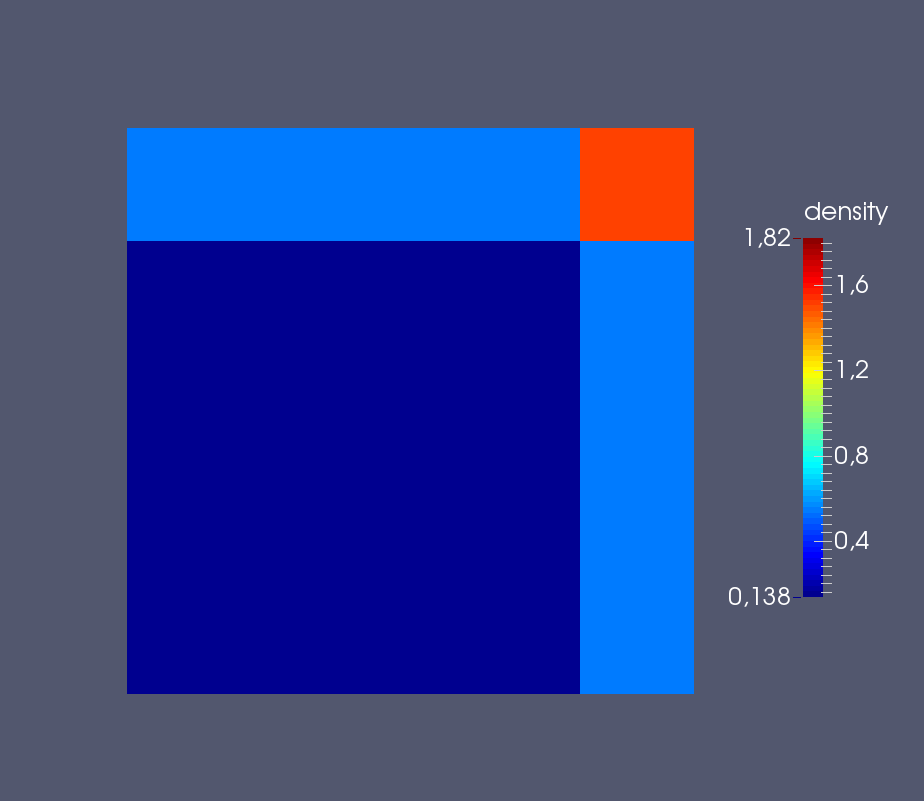
\includegraphics[height=4cm]{images/riemann/riemann_1}
    \hspace{0.1cm}
    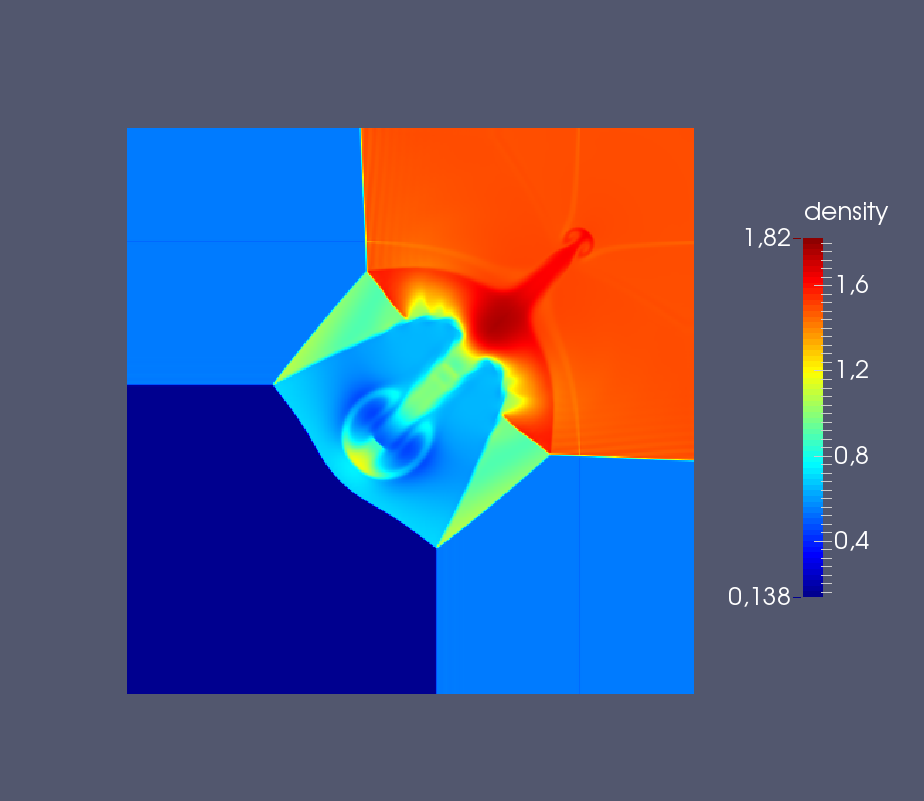
\includegraphics[height=4cm]{images/riemann/riemann_2}
  \end{center}
\end{frame}

%%%%%%%%%%%%%%%%%%%
%% Euler 3D
%%%%%%%%%%%%%%%%%%%
\begin{frame}
\frametitle{Compressible hydrodynamics : Euler equations}

\begin{itemize}
\only<1>{
\item \textbf{\textcolor{blue}{Euler equations}} (conservation of \textbf{mater}, \textbf{momentum} and \textbf{total energy})\begin{align}
  \frac{\partial\rho}{\partial t}+\mathbf{\nabla .}(\rho\mathbf{v}) & = 0\\
  \rho\frac{\partial\mathbf{v}}{\partial t}+\rho(\mathbf{v}.\mathbf{\nabla})\mathbf{v} & =  -\mathbf{\nabla} P\\
  \frac{\partial E}{\partial t} + \mathbf{\nabla}. \left[ (E+P_{tot})\mathbf{v} \right] & =  0
\end{align}}
\only<1>{
\item \textbf{\textcolor{red}{Conservative form}} : %($\partial_t \phi + \nabla \mathbf{f} =  0$) : 
$$ \mathbf{U}_t + \mathbf{F(U)}_x + \mathbf{G(U)}_y + \mathbf{H(U)}_z = \mathbf{0}$$
}
\only<1>{
\item \textcolor{darkgreen}{Conservatives variables and flux}: 
$$\mathbf{U}=\begin{bmatrix}
\rho\\
\rho u\\
\rho v\\
\rho w\\
E 
\end{bmatrix},
\mathbf{F}=\begin{bmatrix}
\rho u\\
\rho u^2+p\\
\rho uv\\
\rho uw\\
u(E+p)
\end{bmatrix},
\mathbf{G}=\begin{bmatrix}
\rho v\\
\rho vu\\
\rho v^2+p\\
\rho vw\\
v(E+p)
\end{bmatrix},
\mathbf{H}=\begin{bmatrix}
\rho w\\
\rho wu\\
\rho wv\\
\rho w^2+p\\
w(E+p)
\end{bmatrix}$$
}
\only<2>{
\item \textbf{\textcolor{red}{Conservative form}} : %($\partial_t \phi + \nabla \mathbf{f} =  0$) : 
%$$ \mathbf{U}_t + \mathbf{F(U)}_x + \mathbf{G(U)}_y + \mathbf{H(U)}_z = \mathbf{0} \Rightarrow \int_{t_n}^{t_{n+1}}\iiint_{C_{i,j,k}} \left( \mathbf{U}_t + \mathbf{F(U)}_x + \mathbf{G(U)}_y + \mathbf{H(U)}_z \right) = \mathbf{0}$$
$$ \mathbf{U}_t + \mathbf{F(U)}_x + ... = \mathbf{0} \Rightarrow \int_{t_n}^{t_{n+1}}\iiint_{C_{i,j,k}} dt \mathbf{dv} \left( \mathbf{U}_t + \mathbf{F(U)}_x + ... \right) = \mathbf{0}$$
\item After \textcolor{blue}{\textbf{time integration}} between $t_n$ and $t_{n+1}$ and over a cell volume :

  \begin{equation*} 
    \frac{\mathbf{U}_{i,j,k}^{n+1}-\mathbf{U}_{i,j,k}^{n}}{\Delta t} +
    \frac{\mathbf{F}_{i+1/2,j,k}^{n+1/2}-\mathbf{F}_{i-1/2,j,k}^{n+1/2}}{\Delta x}  + ... = 0
    %\frac{\mathbf{G}_{i,j+1/2,k}^{n+1/2}-\mathbf{G}_{i,j-1/2,k}^{n+1/2}}{\Delta y}  +
    %\frac{\mathbf{H}_{i,j,k+1/2}^{n+1/2}-\mathbf{H}_{i,j,k-1/2}^{n+1/2}}{\Delta z} = 0
  \end{equation*}
\item \textbf{$\mathbf{U}_{i,j,k}^{n}$ is a volume-averaged quantity at $t_n$}
\item \textbf{$\mathbf{F}_{i+1/2,j,k}^{n+1/2}$ is a time-averaged quantity (between $t_n$ and $t_{n+1}$, explaining index $1/2$) of the surface-average flux at $x=i+1/2$}
\item $E=\rho(\frac{1}{2}\mathbf{V}^2+e)$ Total volumic energy
\item Perfect gas law give the internal energy:
  $e=\frac{p}{\rho(\gamma-1)}$, with $\gamma=1.4$ (ex. air at $T=20^oC$)
\item {\small change to non-conservatives variables: $U \Rightarrow W$ with $^TW=[\rho, u, v, w, p]$}
}
\end{itemize}

\end{frame}

%%%%%%%%%%%%%%%%%%%%%%%%%%%%%%%%%%%%%%%%%%% 
%% Euler 3D
%%%%%%%%%%%%%%%%%%% 
\begin{frame}
  \frametitle{Godunov method - MUSCL-Hancock scheme}
%  
  \only<1>{
    \begin{minipage}{0.55\linewidth}
      \begin{itemize}
      \item $\mathbf{U}_i^{n+1} = \mathbf{U}_i^n+\frac{\Delta
          t}{\Delta x} ( \mathbf{F}_{i-\frac{1}{2}}^{n+1/2}-\mathbf{F}_{i+\frac{1}{2}}^{n+1/2} )$
      \item \textbf{How to compute/approximate flux  $\mathbf{F}_{i-\frac{1}{2}}^{n+1/2}$ ?}
      \item \textbf{\textcolor{red}{1er ordre} Godunov method :}
        % \begin{itemize}
        \item anear $x=i+1/2$, just solve a \textbf{Riemann} problem (Euler system with init conditions defined a \textcolor{red}{piecewise constants} $\mathbf{U}_{i}^{n}$ et $\mathbf{U}_{i+1}^{n}$: $\mathbf{U}^{*}_{i+1/2}=RP(\mathbf{U}_{i}^{n}, \mathbf{U}_{i+1}^{n})$
          \item then use flux $\mathbf{F}_{i+\frac{1}{2}}^{n+1/2} = F(\mathbf{U}^{*}_{i+1/2}(0))$
          \item Many type of Riemann solvers : Roe, HLL, etc ...
            % \end{itemize}
        \end{itemize}
      \end{minipage}
      % 
      \begin{minipage}{0.4\linewidth}
        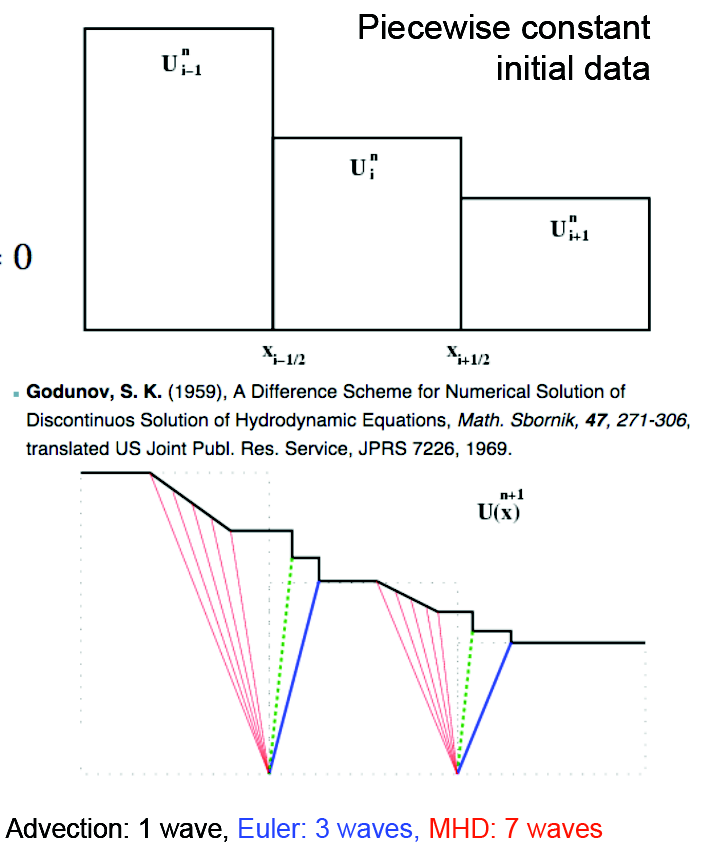
\includegraphics[height=6cm]{./images/godunov}\\
        {\tiny \textbf{Source:} R. Teyssier, 5th JETSET School, \myhref{http://irfu.cea.fr/Projets/COAST/amr_lecture1.pdf}{amr\_lecture1.pdf}\\
        book: \textit{Riemann Solvers And Numerical Methods for Fluid Dynamics: A Practical Introduction}, by E. F. Toro, Springer }
      \end{minipage}
    }
\only<2>{
\begin{minipage}{0.5\linewidth}
  \textbf{MUSCL-Hancock} (Monotone Upstream-centered Schemes for Conservation Laws) scheme implemented
\end{minipage}
\begin{minipage}{0.45\linewidth}
  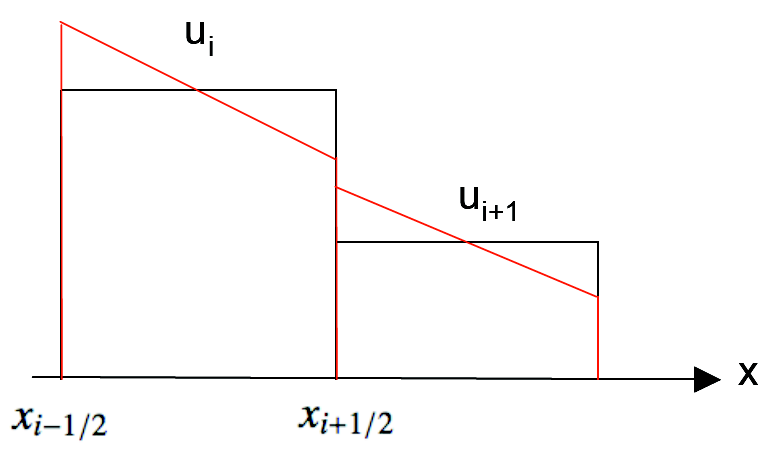
\includegraphics[height=2.8cm]{./images/godunov_2nd_ordre}\\
\end{minipage}
\begin{itemize}
\item 2nd order Godunov scheme : $\mathbf{U}_i^n$ replaced by linear picewise functions(predictor-corrector scheme).
\item MUSCL-Hancock done in 3 steps : \\
- compute slopes $\Delta_i$ (using a TVD limiter) and extrapolate $\mathbf{U_i}$ values to cell edges\\
- perform 1/2 time step integration of edge values\\
- solve Riemann problems at cell interfaces to get fluxes
$\mathbf{F_{i+\frac{1}{2}}}$, then update $\mathbf{U_i}$ at next time step
\end{itemize}
}
\end{frame}

%%%%%%%%%%%%%%%%%%%%%%%%%%%%%%%%%%%%%%%%%%%
%%%%%%%%%%%%%%%%%%%%%%%%%%%%%%%%%%%%%%%%%%%
% \begin{frame}
%   \frametitle{Sch\'ema num\'erique s\'epar\'e en direction}
% On remplace :\\
% \begin{equation*}
%   \left.
%   \begin{array}{r l}
%     \text{\textcolor{darkblue}{EDP}}  &  \quad \mathbf{U}_t + \mathbf{F(U)}_x + \mathbf{G(U)}_y + \mathbf{H(U)}_z = 0\\
%     \text{\textcolor{darkblue}{CI}}   & \quad \mathbf{U}(x,y,z,t^n)=\mathbf{U}_{i,j,k}^n\\
%     \end{array} \right\} \Rightarrow\mathbf{U}^{n+1}
% \end{equation*}
% par\\
% \begin{equation*}
%   \left.
%   \begin{array}{r l}
%     \text{\textcolor{darkblue}{EDP}}  & \quad \mathbf{U}_t + \mathbf{F(U)}_x = 0\\
%     \text{\textcolor{darkblue}{CI}}   & \quad \mathbf{U}_{i,j,k}^n \\
%   \end{array} \right\} \Rightarrow\mathbf{U}^{n+1/3}
% \end{equation*}
% %
% \begin{equation*}
%   \left.
%   \begin{array}{r l}
%     \text{\textcolor{darkblue}{EDP}}  & \quad \mathbf{U}_t + \mathbf{G(U)}_y = 0\\
%     \text{\textcolor{darkblue}{CI}}   & \quad \mathbf{U}_{i,j,k}^{n+1/3} \\
%   \end{array} \right\} \Rightarrow\mathbf{U}^{n+2/3}
% \end{equation*}
% %
% \begin{equation*}
%   \left.
%   \begin{array}{r l}
%     \text{\textcolor{darkblue}{EDP}}  & \quad \mathbf{U}_t + \mathbf{H(U)}_z = 0\\
%     \text{\textcolor{darkblue}{CI}}   & \quad \mathbf{U}_{i,j,k}^{n+2/3} \\
%   \end{array} \right\} \Rightarrow\mathbf{U}^{n+1}
% \end{equation*}
% \end{frame}


%%%%%%%%%%%%%%%%%%%%%%%%%%%%%%%%%%%%%%%%%%%
%% Structures de donn\'ees
%%%%%%%%%%%%%%%%%%%
\begin{frame}
\frametitle{Data Structures}

\begin{itemize}
\item Four 2D grids:
  \begin{itemize}
  \item 1 per conservative variable : $\rho$, $\rho v_x$, $\rho v_y$, $e$
  \item 2d space discretization
  \item limit conditions : 2 ghost cells, multiple types
    \begin{itemize}
    \item reflective
    \item absorbing
    \item periodic
    \end{itemize}
  \end{itemize}
\end{itemize}

\begin{center}
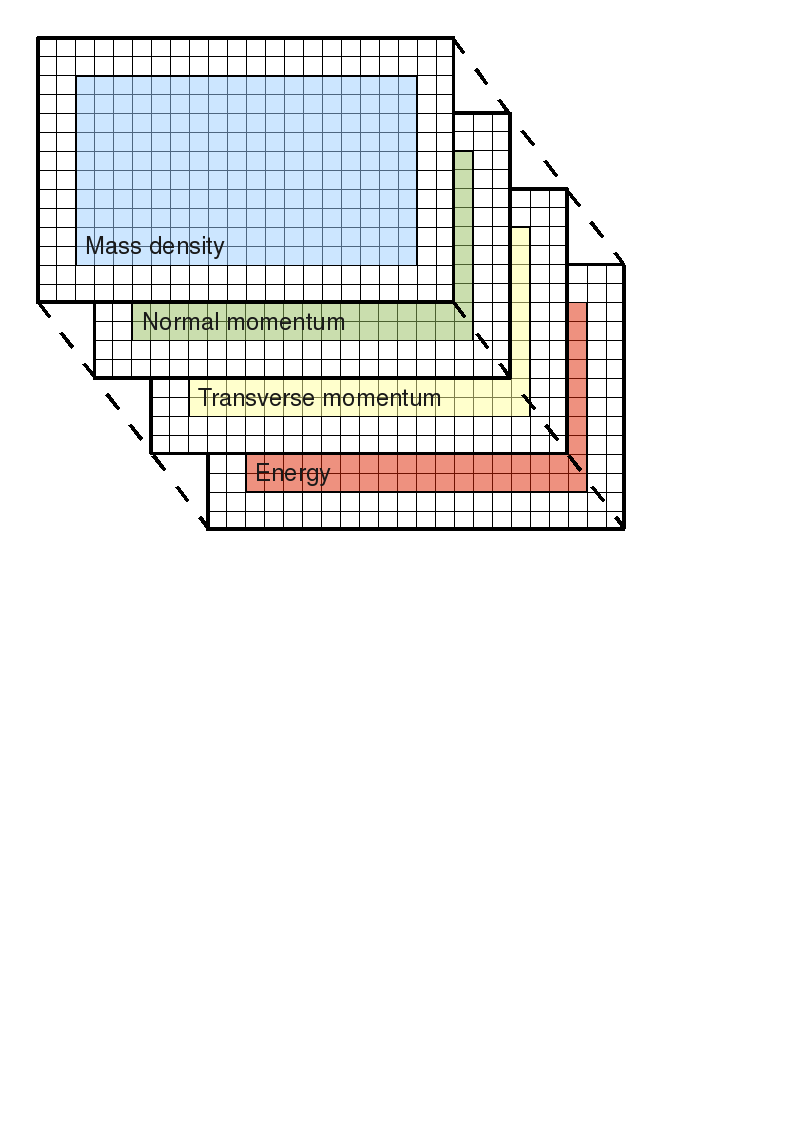
\includegraphics[height=10cm]{./images/Arrays}
\end{center}

\end{frame}

%%%%%%%%%%%%%%%%%%%%%%%%%%%%%%%%%%%%%%%%%%%
%% Simulation
%%%%%%%%%%%%%%%%%%%
\begin{frame}
\frametitle{Simulation}

\begin{itemize}
\item jet simulation
\item parameters 
\begin{itemize}
\item run parameters (total time, output rate)
\item geometric parameters (NX, NY, $\Delta x$)
\item border types
\item schmeme parameters
\item jet parameters
\end{itemize}
\end{itemize}

\begin{center}
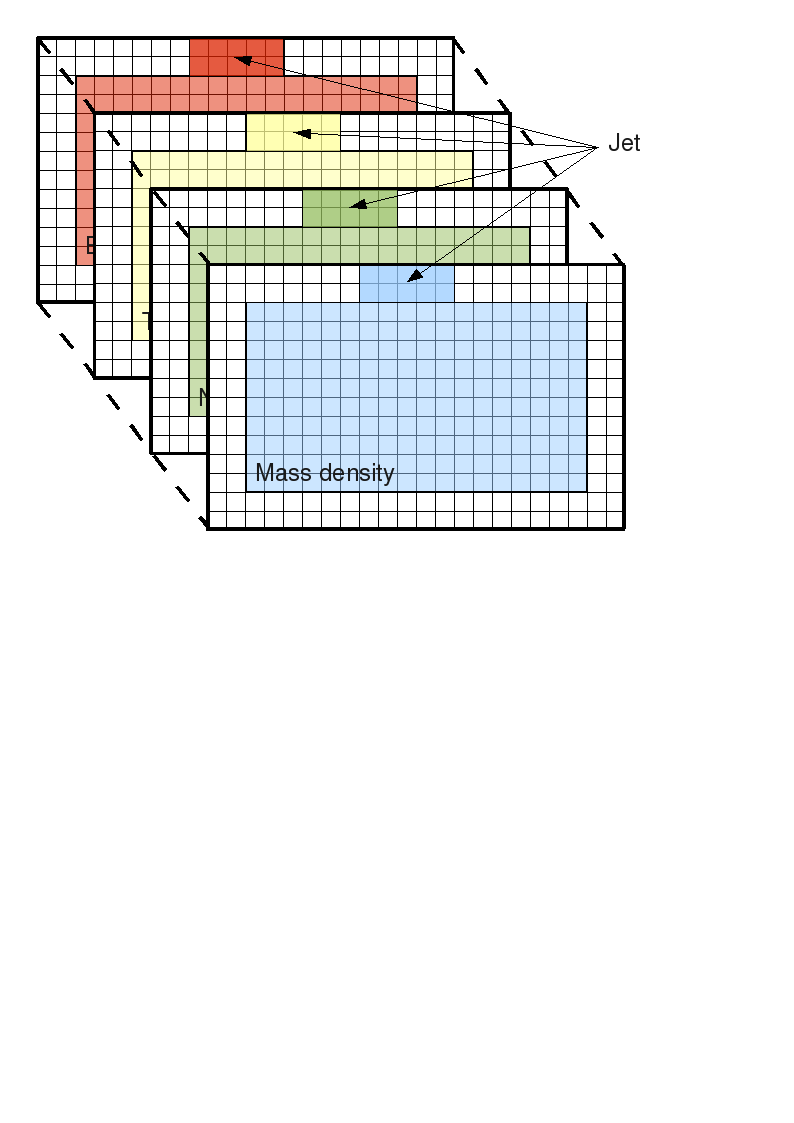
\includegraphics[height=10cm]{./images/Jet}
\end{center}

\end{frame}

%%%%%%%%%%%%%%%%%%%%%%%%%%%%%%%%%%%%%%%%%%%
%% Version s\'equentielle
%%%%%%%%%%%%%%%%%%%%%%%%%%%%%%%%%%%%%%%%%%%
\begin{frame}
\frametitle{Sequential version of \texttt{Euler2D}}

\begin{itemize}
\item How to run ?
  \texttt{./euler2d.cuda ./test.ini}
\item Quick output visualization: paraview
%\item description de l'implantation de l'algorithme de Godunov
%\item description des structures de donn\'ees
\end{itemize}

\end{frame}

%%%%%%%%%%%%%%%%%%%%%%%%%%%%%%%%%%%%%%%%%%%
%% Visualisation
%%%%%%%%%%%%%%%%%%%%%%%%%%%%%%%%%%%%%%%%%%%
\begin{frame}
\frametitle{Visualisation}

\begin{itemize}
\item File format is \myhref{http://www.vtk.org/}{VTK}: more precisely VTI (for regular cartesian grids)~\footnote{vtr format is also possible here.}; see website \myhref{http://www.cacr.caltech.edu/~slombey/asci/vtk/vtk_formats.simple.html}{vtk\_formats.simple.html} which describes VTK files format variants
\item Visualization GUI: 
  \begin{itemize}
  \item \myhref{http://www.paraview.org/}{paraview}
  \item Can also use standalone python script \texttt{plot\_data.py}
  \end{itemize}
\end{itemize}

\end{frame}

%%%%%%%%%%%%%%%%%%%%%%%%%%%%%%%%%%%%%%%%%%%
%% Reference
%%%%%%%%%%%%%%%%%%%%%%%%%%%%%%%%%%%%%%%%%%%
\begin{frame}
  \frametitle{Additional reference}
  
  \begin{itemize}
  \item See C.P. Dullemond document on CFD numerical methods: {\small \myurl{http://www.mpia-hd.mpg.de/~dullemon/lectures/fluiddynamics08/}}
  \end{itemize}

\end{frame}
